\documentclass[11pt,a4paper]{article}

\usepackage{fontspec}
\usepackage{xeCJK}
\setCJKmainfont{GenRyuMin2 TW}
\setCJKsansfont{GenSekiGothic2 TC}
\xeCJKsetup{CJKmath=true}

\usepackage[margin=2.4cm]{geometry}
\usepackage{parskip}
\usepackage{graphicx}
\graphicspath{{../../figures/cautionary/}}
\usepackage{amsmath,amssymb}
\usepackage{booktabs}
\usepackage{caption}
\usepackage{xcolor}
\usepackage{enumitem}
\usepackage[colorlinks=true,linkcolor=blue,citecolor=blue,urlcolor=blue]{hyperref}
\usepackage{authblk}

\title{\bfseries 擾動單細胞 RNA 定序之拓撲資料分析的結構感知對照：\\
共變異數匹配虛無模型、繞行檢定，與一則警示案例}
\author[1]{林\,H.-T.}
\author[1]{涂\,Y.-H.}
\affil[1]{\small 預印本——方法學報告。程式碼：\url{https://github.com/htlin222/sctda-cancer-plasticity}}
\date{\today}

\newcommand{\maxh}{\ensuremath{\max\text{-}H_1}}

\begin{document}
\maketitle

\begin{center}
\fbox{\begin{minipage}{0.94\linewidth}\small
\textbf{重點摘要。}
\begin{itemize}[leftmargin=1.2em,itemsep=1pt,topsep=2pt]
\item 一個熱門的拓撲統計量——\maxh，即最具持續性之「環」的大小——\emph{看似}在量化環狀的藥物耐受可塑性，
且在五個癌症系統中隨藥物上升。
\item 它通不過三道簡單對照：細胞從未繞行該環；基線訊號只是資料的散佈（離散度）；藥物誘發的部分是細胞週期
（其本身就是一個環）。
\item 我們把這些對照打包成一套可重複使用的檢查（圖~\ref{fig:flow}），在合成資料上驗證，並以我們自己的分析
示範這個陷阱。
\item \textbf{要點：} 在把任何「持續性大小的差異」讀作生物學之前，先跑這套檢查。
\end{itemize}
\end{minipage}}
\end{center}

\begin{abstract}
\noindent 隨著拓撲資料分析（TDA）進入單細胞生物學，持續同調的純量摘要——最簡單者為最大一維持續性
（\maxh）——開始被讀作「環狀（cyclic）」細胞狀態結構的量化指標，並被拿來跨條件比較。這有兩個各自已知、
但在實務上未被同時控制的危險：在 Vietoris--Rips 濾流中，持續性的「大小」即使在純噪音下也會隨點雲的散佈
（離散度）與取樣而增長 [3]；而細胞週期本身就是表達空間中的一個環 [1,5]。我們將四道對照整合成一套可重複使用
的、適用於擾動 scRNA-seq 的顯著性程序——(i)~一個保留轉錄離散度的\textbf{共變異數匹配高斯虛無模型}；
(ii)~一個在做任何環狀詮釋之前、先問該環是否被細胞「佔據」的\textbf{圓形座標繞行檢定}；(iii)~\textbf{相對於
離散度虛無模型}而非以原始持續性來評估的\textbf{細胞週期回歸}；以及 (iv)~\textbf{自助法方向性檢定}——並在
已知真值的合成資料上驗證（對真正被繞行的環敏感；對良性離散度與非高斯、非環狀結構具特異性）。作為警示案例，
我們報告我們自己對五個縱向 EGFR 突變肺癌系統的分析：一個看似可信、可重現、跨尺度、與藥物相關的 \maxh{}
訊號，在這些對照下瓦解——細胞從未繞行該環（$R \ge 0.965$，相較於 12\% 被佔據之對照的 $0.881$）、基線
\maxh{} 等於離散度虛無模型、而體外的藥物超額其實是細胞週期環。該框架在真結構存在處亦能將其分離出來——
PDX 殘存病灶中一個藥物誘發的多纖毛程式——顯示它同時能通過真訊號、也能拒絕被混淆的訊號。我們建議：隨著
純量 TDA 讀數在單細胞生物學中日益普及，應將這些對照列為標準做法，並以開源程式碼釋出。
\end{abstract}

\paragraph{貢獻與和既有工作的關係。} 各個混淆因子與若干補救方法皆為已知；我們的貢獻在於將它們
\emph{整合成一套適用於單細胞 $H_1$ 的校正顯著性程序}，附帶一個經驗證的操作點，外加一個誠實的失敗案例。
\begin{enumerate}[leftmargin=1.4em,itemsep=1pt]
\item 一個適用於 scRNA-seq \maxh{} 的\textbf{共變異數匹配高斯虛無模型}，用以控制離散度。主流已發表的
scTDA 虛無模型是「細胞內基因標籤洗牌」[1]，它會摧毀共變異數、因而幾乎被任何真實資料超越；TDA 理論面上更
合理的替代是子取樣信賴集 [4]。一個保留離散度的虛無模型用於單細胞持續性，似乎尚未被使用過，儘管在嵌入幾何
的「弱對照 vs 強對照」批判中已有先例 [9]。
\item 一個\textbf{圓形座標繞行檢定} [10]，將「環被佔據」確立為任何「環狀」詮釋的前提。
\item 明確指出：\textbf{以「原始 \maxh{} 在 S/G2M 回歸後仍存在」為依據的細胞週期對照是不充分的}，因為原始
持續性被離散度主導 [3]；細胞週期的貢獻必須相對於離散度虛無模型來判斷。細胞週期成環的混淆本身已被確立
[1,5]；而原始持續性對照之不充分，據我們所知，尚未被指出。
\item 一個刻畫敏感度與特異度的\textbf{合成基準}，以及一個五系統的\textbf{警示案例}——我們自己的——其中一個
被混淆的訊號可重現、跨尺度、卻是錯的，證明這個陷阱對謹慎的研究者而言是真實的。
\end{enumerate}

\section{引言}
拓撲資料分析正進入單細胞生物學，已有綜述在彙整持續同調與 Mapper 應用於 scRNA-seq 的案例 [8]。其魅力在於能
偵測軌跡推斷工具（為單向進程而設計）所無法量化的封閉、非樹狀結構（環；一維同調 $H_1$）。隨著領域成熟，一個
自然的步驟是以純量摘要拓撲——\maxh、總持續性、持續性熵——並跨條件比較，將其上升讀作更多的環狀結構或可塑性。
在癌症藥物耐受中這格外誘人：譜系追蹤顯示持續細胞會在多種狀態間可逆轉換，這種行為很容易被稱作「環狀」。

我們主張這一步需要當前實務未同時施加的對照，並提供之。兩個混淆因子各自皆有文獻記載。其一，Vietoris--Rips
持續性對點雲的散佈與取樣密度敏感：純隨機點的「最大持續環」會隨樣本數增長 [3]，原始持續性的大小與度量／尺度
相關（因而催生了如持續性影像與持續性地景等穩定化摘要 [6,7]）且對離群值敏感（因而催生了密度穩健的濾流
[8b]）。擾動下轉錄離散度的上升因此可在真拓撲毫無改變時抬高 \maxh。其二，細胞週期在表達空間中描出一個圓
[5]，是 scRNA-seq 中 $H_1$ 環的典型生成者；領域奠基的 scTDA 方法明言「細胞週期會在表達空間中產生週期性結構」
[1]。常用的虛無模型並未控制前者（基因標籤洗牌 [1] 會摧毀包含離散度在內的共變異數），而一篇近期綜述指出單細胞
TDA「可能不提供嚴謹的統計評估」、且對前處理敏感，卻未予解決 [8]。

這是一個\emph{預防性}的貢獻，並非主張一個普遍的錯誤正在被犯：在 scRNA-seq 上做純量持續性對條件的比較仍不
常見（既有的 scTDA 方法使用 Mapper 圖與逐細胞特徵 [1,2]），且已有控制樣本數並使用圖距離的謹慎應用 [11]。
我們的重點是：當「純量讀數」這一步變得吸引人時，下述對照應隨之而來——而且這個陷阱是真實的，因為我們自己就掉
了進去。我們以我們自己的五系統分析作為警示範例。

\section{結果}
\subsection*{對照框架}
用白話說（圖~\ref{fig:flow}）：持續性的「大小」就是資料中最穩固的「環」有多大，但一個「環」可能是被細胞變得
更分散（離散度）或被細胞週期（表達空間中的一個圓）偽造出來的；因此我們依序問三個問題——環有沒有比單純的分散
更多？細胞有沒有真的繞著它走？剩下的是不是只是細胞週期？對每個條件，回報三個量加上一條決策規則。(1)~\emph{離散度檢定}：觀測 \maxh{} 與「對嵌入之均值與共變異數匹配
的多元高斯」之 \maxh{} 的比值；比值接近 1 表示該統計量可由離散度解釋，穩健地 $>1$ 則表示存在超越離散度的
結構。(2)~\emph{繞行檢定}：取自最具持續性之 $H_1$ 類的圓形座標 [10] 之 Rayleigh 集中度 $R$；$R$ 接近 1 表示
族群擠在單一角度（環未被佔據）。(3)~\emph{細胞週期檢定}：在 S/G2M 分數回歸 [12] 後重算離散度比值。三者皆以
自助法子取樣包裹 [4]；結論建立在「某個排序在多少比例的子取樣中成立」之上。決策規則：若高斯比值穩健地 $>1$ 則
為\emph{超越離散度的結構}；唯有同時 $R<0.6$ 才是\emph{被繞行的環}；若超額在 S/G2M 回歸後不存活則為
\emph{細胞週期驅動}。

\subsection*{框架在合成真值上兼具敏感度與特異度}
在答案已知的點雲上（各 n=1{,}200，結構置於二維、嵌入 30 維並加上各向同性噪音；\textbf{圖 4}）：高斯團塊得到
比值 0.93、$R=0.99$（正確判為\emph{無結構}）；均勻被繞行的環得到比值 8.35、$R=0.42$（正確判為\emph{被繞行的
環}；敏感度）；稀疏非閉合弧得到比值 1.54、$R=0.96$（\emph{有結構但未被繞行}）；兩個分離的高斯團——非高斯但
非環狀——得到比值 0.93（\emph{無結構}；特異度）。高斯虛無模型不會對良性的非高斯性產生偽陽性，這正是對共變異數
匹配虛無模型最關鍵的反對意見。第二個非參數、保留離散度的虛無模型（逐主成分置換）與之一致且更為保守。

\subsection*{案例研究：一個看似存在的藥物耐受拓撲訊號}
我們在五個 EGFR 突變系統上計算 \maxh（前 30 主成分，$\mathbb{F}_2$）。\maxh{} 在 osimertinib 細胞株與 PDX
模型中隨藥物上升（osimertinib D0$\to$D14 為 $1.41\to3.78$；PDX YU-006 未治療$\to$殘存為 $2.79\to5.46$；
\textbf{圖 1}）。erlotinib 序列在此階段已是反例——訊號弱且非單調（D9 為 1.77、D11 為 1.08，是該序列最低）。

\subsection*{對照一——細胞並未繞行該環}
圓形座標在每個世代中皆塌縮至單一角度：Rayleigh $R \ge 0.965$（\textbf{圖 2a}）——比 12\% 被佔據之陽性對照的
$R=0.881$ 還要集中。譜系（Watermelon 條碼）若有不同，反而比隨機\emph{更}集中。該環是一個族群並未佔據或繞行
的稀疏特徵。

\subsection*{對照二——基線 \maxh{} 即離散度}
對共變異數匹配高斯虛無模型而言，基線 \maxh{} 並未超越離散度（osimertinib D0/D3 比值 $\approx 0.9$；觀測
$>$ 虛無模型者僅占 18--31\% 的子取樣；\textbf{圖 1}）。超額僅在藥物下出現（osimertinib D7/D14 為 100\%/98\%；
PDX 殘存為 99\%）。由於高斯僅保留二階動差，其失效模式對「否定性結論」而言是保守的。

\subsection*{對照三——體外超額是細胞週期；體內超額不是}
osimertinib D14 的超額由增殖細胞貢獻（差異表達：PTTG1、UBE2S、CKS1B、MYBL2；增殖標記 MKI67/PCNA/CCNB1/CDK1/
BIRC5，5/6），且在 S/G2M 回歸後不存活：D14 比值由 1.18$\to$0.99，且 D14 $>$ D0 僅在 31\% 的自助法中成立
（\textbf{圖 2b}）。常見的對照——\emph{原始} \maxh{} 在回歸後仍存在——會錯誤地下結論「不是細胞週期」，因為
原始 \maxh{} 被離散度主導 [3]。該框架是「分解」而非一律「拆穿」：在體內的 PDX 中，殘存超額\emph{並非}細胞週期
（去除增殖細胞後的 G1-only 比值為 2.07，90\% CI $[1.37,2.61]$，在 100\% 的自助法中 $>1$），但仍未通過繞行檢定
（$R=0.965$）。橫跨全部五個系統：離散度解釋基線；細胞週期解釋體外超額；體內殘存則是真實但未被繞行——而在
任何系統中，\maxh{} 都未能佐證一個被細胞繞行的環（表~\ref{tab:summary}）。

\begin{table}[h]\centering\small
\caption{各系統在每道對照下的結果。}\label{tab:summary}
\begin{tabular}{@{}lllll@{}}\toprule
系統 & 離散度 & 繞行 $R$ & 細胞週期 & 判決 \\\midrule
osimertinib 細胞株 & 基線 $\approx$1、藥物 1.4 & 0.997（否） & 超額\emph{是}細胞週期 & 被混淆 \\
PDX（YU-006） & 藥物 1.95 & 0.965（否） & 超額\emph{非}細胞週期 & 真實、未被繞行 \\
erlotinib 細胞株 & $\approx$1（無超額） & --- & --- & 無訊號 \\
病人腫瘤 & 基線也有超額 & 高 & 不適用 & 異質性 \\\bottomrule
\end{tabular}
\end{table}

\subsection*{一個抗混淆的譜系統計量在標準資料上力量不足}
一個對抗譜系洗牌虛無模型的譜系狀態記憶統計量 $M(t)=1-H_{\mathrm{obs}}/H_{\mathrm{null}}$ 在 Watermelon 資料
上並不穩健：基線的下降「被暗示」但不穩健（M(D0) 點估計 0.48，但 90\% CI 為 $[-0.05,0.29]$，且跨越零），而其
在藥物下的衰減在不同分群設定下會\emph{變號}（9 種設定中僅 3 種為正）、非單調，並在深度分層虛無模型下減半
（\textbf{圖 3}）。原因是力量：每個時間點僅有 12--33 個含 $\ge 3$ 個細胞的克隆。

\subsection*{超越拒絕：框架能分離出一個真實、可詮釋的程式}
一個對照框架唯有在「能通過真結構」時才值得信任（參見合成的真陽性）。PDX 殘存即為實例：其超額——唯一通過所有
對照的訊號——由一個連貫的多纖毛氣道上皮程式驅動（PIFO、RSPH1、CFAP45/126/157、CAPS/CAPSL、CETN2、TPPP3；
分泌性 AGR2/AGR3），在 YU-006 中為藥物誘發（未治療細胞中 0.1\% $\to$ 殘存病灶中 9.6\%；絕對數約 6 $\to$ 約
187 個細胞，同時腫瘤體積縮小三倍），與 EGFR-TKI 持續細胞已知會採取的分化譜系狀態一致。兩個界線：該程式具
模型專一性（在 YU-003 中不存在），且在缺乏匹配正常參照的情況下，拷貝數推斷無法判定這些纖毛細胞是腫瘤來源
（轉分化）還是被擴增的非惡性族群。此真實結構仍未通過繞行檢定。

\section{方法}
GEO GSE134839/150949/243562/131907 加 Maynard 2020；scanpy 之 QC／HVG／PCA（種子 42），子取樣至 1{,}000--
1{,}500 個細胞；\texttt{ripser} 0.6 之 Vietoris--Rips 至 $H_1$，於前 30 主成分（$\mathbb{F}_2$）。離散度虛無模型：
自嵌入點雲的 $\mathcal{N}(\hat\mu,\hat\Sigma)$ 抽樣，比值 $=$ 觀測值／虛無模型中位數，30 次自助法子取樣加 90\%
信賴區間，第二虛無模型為逐主成分置換。繞行檢定：\texttt{dreimac} 之 \texttt{CircularCoords}（DSPVJ [10]），
Rayleigh $R$（驗證：噪音圓 $R=0.12$；12\% 被佔據之環 $R=0.88$）。細胞週期檢定：留一群、Wilcoxon 差異表達、
S/G2M 回歸 [12]，並以自助法重算離散度比值。體內身分：對原始計數做差異表達、跨 PDX 評分纖毛特徵、以
\texttt{infercnvpy} 做 CNV。程式碼：\texttt{scripts/16\_*.py}--\texttt{scripts/27\_*.py}（MIT）。

\section{討論}
一個跨系統的藥物耐受拓撲訊號——上升的 \maxh——大致由轉錄離散度、以及在體外由細胞週期所解釋；而在仍存有真正
非混淆結構之處，它依然無法佐證環狀可塑性，因為族群並未繞行它。這個看似訊號者在五個系統中看來都很有說服力、
通過了一個「已發表式」的細胞週期對照、並在病人腫瘤中「重現」——這正是這些對照之所以重要的原因：一個被混淆的
統計量可以同時可重現、跨尺度、而且是錯的。我們的貢獻是預防性且整合性的。各混淆因子皆有先前文獻——持續性對
密度／樣本數的依賴 [3]、細胞週期環 [1,5]、單細胞 TDA 的前處理敏感性與缺乏顯著性檢定 [8]，以及最接近我們論點
者：在單細胞基礎模型嵌入中，於弱（洗牌）對照下顯著的幾何結構，在更強對照下會消失 [9]。我們在標的與虛無模型
上不同（原始表達 $H_1$ 加共變異數匹配高斯虛無模型，相對於嵌入幾何加重連線虛無模型），並貢獻了將離散度虛無
模型、繞行檢定、與相對於離散度的細胞週期對照\emph{整合}成單一、經真值驗證之程序。該框架亦浮現出殘存病灶中一個
藥物誘發的多纖毛程式；其是否為賦予耐受性的腫瘤轉分化，是一個前瞻性、需實驗承載的研究計畫，而非重新分析。

\paragraph{展望。} 要使此體內程式成為一項發現，需解決細胞來源（匹配正常之 CNV 或 EGFR 驅動基因定型）、在更多
模型或病人殘存病灶檢體中重現，以及功能性測試該分化狀態是否賦予耐受。
\paragraph{限制。} 細胞週期歸因僅在 osimertinib 細胞株上示範；PDX 殘存超額已證明非細胞週期，但其細胞來源未解。
我們處理的是 \maxh；離散度虛無模型源自同一濾流，理應可推廣至其他持續性摘要 [6,7] 與更高維同調，惟此處未測。

\begin{figure}[t]\centering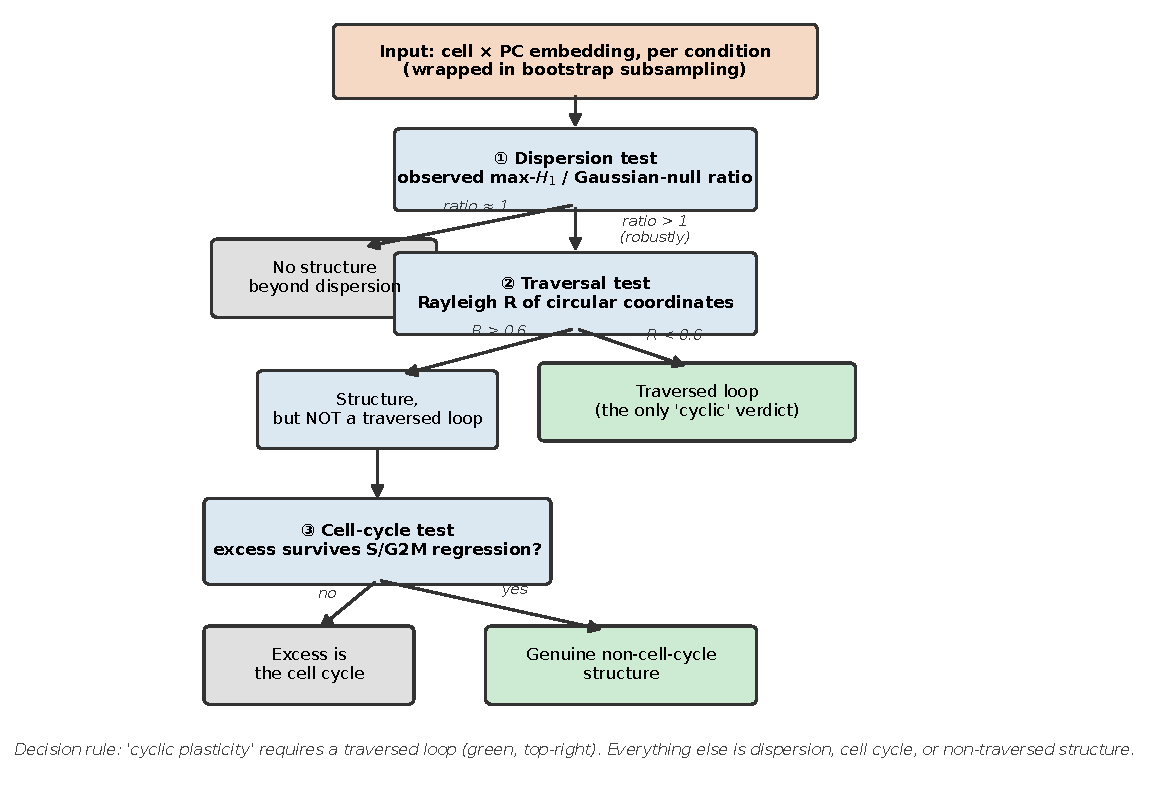
\includegraphics[width=0.92\linewidth]{fig5_framework_flowchart.pdf}
\caption{框架作為一棵決策樹：輸入 $\to$ 離散度檢定 $\to$ 繞行檢定 $\to$ 細胞週期檢定 $\to$ 判決（綠色＝真結構；
灰色＝偽影）。「環狀可塑性」需要一個被繞行的環；其餘皆為離散度、細胞週期、或未被繞行的結構。}\label{fig:flow}\end{figure}

\begin{figure}[t]\centering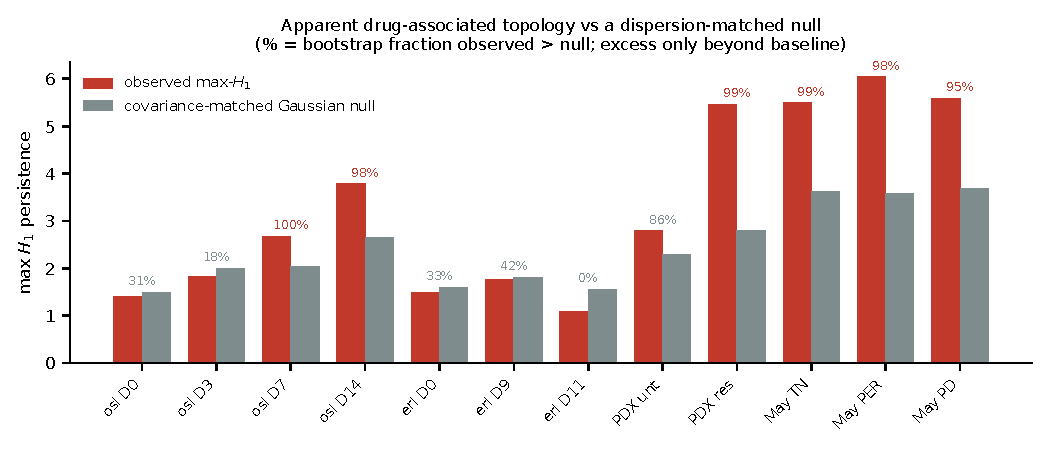
\includegraphics[width=\linewidth]{fig1_dispersion_null.pdf}
\caption{觀測 \maxh{} 對共變異數匹配高斯（離散度）虛無模型，橫跨五個系統。百分比：觀測 $>$ 虛無模型的自助法
比例。超額僅在藥物下出現。}\label{fig:disp}\end{figure}
\begin{figure}[t]\centering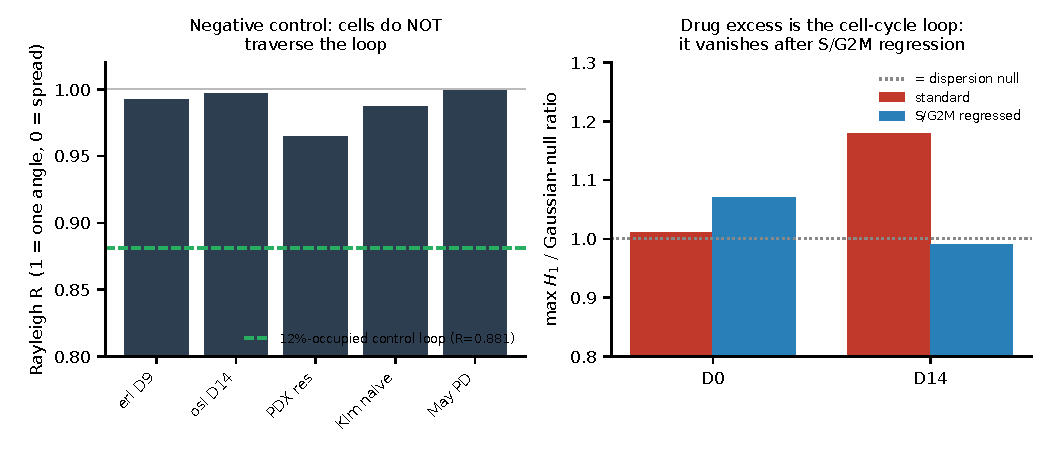
\includegraphics[width=\linewidth]{fig2_controls.pdf}
\caption{(a)~繞行檢定：所有世代 $R\ge0.965$，相較於 12\% 被佔據之對照的 $0.881$。(b)~體外藥物超額在 S/G2M
回歸後消失。}\label{fig:ctrl}\end{figure}
\begin{figure}[t]\centering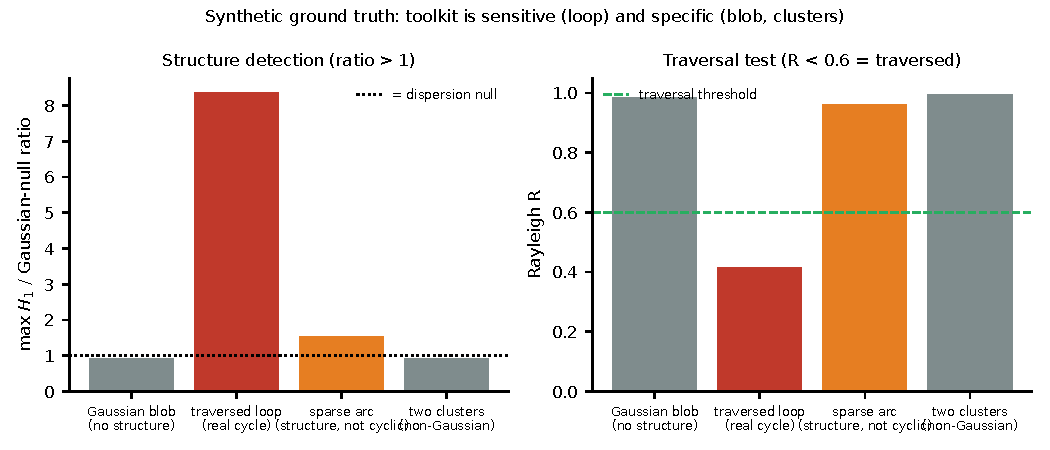
\includegraphics[width=\linewidth]{fig4_synthetic_benchmark.pdf}
\caption{合成真值：框架兼具敏感度（通過被繞行的環）與特異度（拒絕高斯團塊與雙團非高斯案例）。}\label{fig:bench}\end{figure}
\begin{figure}[t]\centering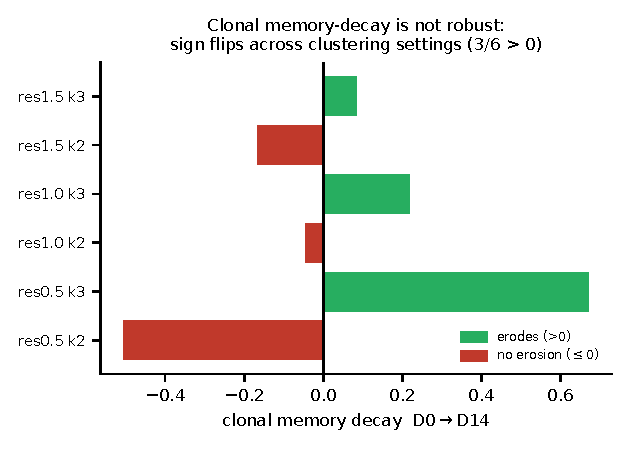
\includegraphics[width=0.62\linewidth]{fig3_memory_nonrobust.pdf}
\caption{譜系記憶衰減並不穩健：D0$\to$D14 的變化在不同分群設定下變號。}\label{fig:mem}\end{figure}

\begin{thebibliography}{99}\small
\bibitem{r1} Rizvi AH, C\'amara PG, Kandror EK, et al. Single-cell topological RNA-seq analysis. \emph{Nat Biotechnol} 2017;35:551--560.
\bibitem{r2} Nicolau M, Levine AJ, Carlsson G. Topology based data analysis identifies a breast-cancer subgroup. \emph{PNAS} 2011;108:7265--7270.
\bibitem{r3} Bobrowski O, Kahle M, Skraba P. Maximally persistent cycles in random geometric complexes. \emph{Ann Appl Probab} 2017;27:2032--2060.
\bibitem{r4} Fasy BT, Lecci F, Rinaldo A, Wasserman L, et al. Confidence sets for persistence diagrams. \emph{Ann Statist} 2014;42:2301--2339.
\bibitem{r5} Schwabe D, Formichetti S, Junker JP, Falcke M, Rajewsky N. The transcriptome dynamics of single cells during the cell cycle. \emph{Mol Syst Biol} 2020;16:e9946.
\bibitem{r6} Adams H, Emerson T, Kirby M, et al. Persistence images. \emph{JMLR} 2017;18:1--35.
\bibitem{r7} Bubenik P. Statistical TDA using persistence landscapes. \emph{JMLR} 2015;16:77--102.
\bibitem{r8} Hern\'andez-Lemus E. Topological data analysis in single cell biology. \emph{Front Immunol} 2025;16:1615278.（8b：Chazal F, et al. Robust topological inference / DTM filtrations. \emph{JMLR} 2017;18:1--40.）
\bibitem{r9} Kendiukhov I. What topological and geometric structure do biological foundation models learn? \emph{arXiv} 2026;2602.22289.
\bibitem{r10} de Silva V, Morozov D, Vejdemo-Johansson M. Persistent cohomology and circular coordinates. \emph{Discrete Comput Geom} 2011;45:737--759.
\bibitem{r11} Mukherjee S, Wethington D, Dey TK, Das J. Clinically relevant features in cytometry via persistent homology. \emph{PLoS Comput Biol} 2022;18:e1009931.
\bibitem{r12} Tirosh I, Izar B, Prakadan SM, et al. Dissecting metastatic melanoma by single-cell RNA-seq. \emph{Science} 2016;352:189--196.
\end{thebibliography}

\end{document}
